\begin{frame}{The BNP Model}
A {\bf Dirichlet process prior} allows for an infinite number of components.
\vspace{-0.2in}
\begin{figure}[!h]
\centering
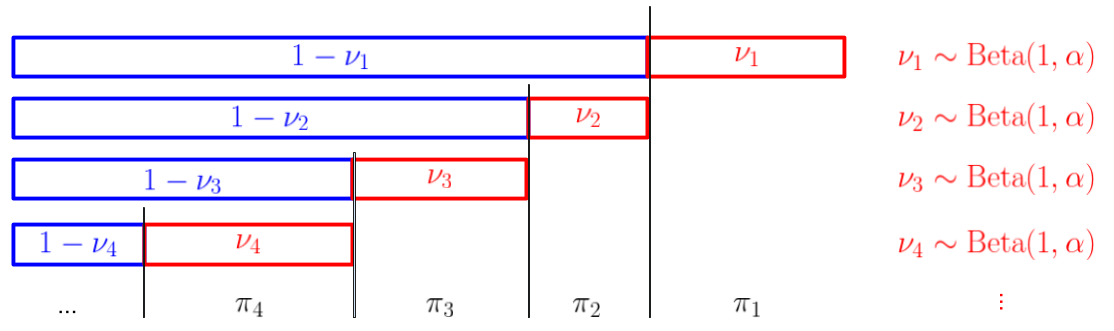
\includegraphics[width = 0.95\textwidth]{./figures/DP_stick_breaking.png}
\caption{A schematic of the Dirichlet process prior}
\end{figure}
\vspace{-0.2in}

While there are an infinite number of {\bf components}, there are a finite number of {\bf clusters} in a given dataset. \pause We might ask:

\begin{enumerate}[(1)]
\item How many clusters are in the {\itshape current} dataset?

\pause
\item Given our current knowledge, how many clusters would we expect to see in a {\itshape new} dataset?

\end{enumerate}

\pause

These quantities depend on the choice of stick-breaking prior.

\pause

\begin{mdframed}[style=MyFrame]
\begin{center}
{\bf What makes this stick-breaking prior a reasonable one?}
\end{center}
\end{mdframed}

\end{frame}
